\documentclass[ignorenonframetext,]{beamer}
\usetheme{AnnArbor}
\usecolortheme{beaver}
\usefonttheme{structurebold}
\setbeamertemplate{caption}[numbered]
\setbeamertemplate{caption label separator}{: }
\setbeamercolor{caption name}{fg=normal text.fg}
\usepackage{amssymb,amsmath}

% required for kable and kableExtra for R  ----
\usepackage{longtable}
\usepackage{booktabs} 
% < --- < ---

\usepackage{ifxetex,ifluatex}
\usepackage{fixltx2e} % provides \textsubscript
\usepackage{lmodern}
\usepackage{xeCJK}
\ifxetex
  \usepackage{fontspec,xltxtra,xunicode}
  \defaultfontfeatures{Mapping=tex-text,Scale=MatchLowercase}
  \newcommand{\euro}{€}
\else
  \ifluatex
    \usepackage{fontspec}
    \defaultfontfeatures{Mapping=tex-text,Scale=MatchLowercase}
    \newcommand{\euro}{€}
  \else
    \usepackage[T1]{fontenc}
    \usepackage[utf8]{inputenc}
      \fi
\fi
% use upquote if available, for straight quotes in verbatim environments
\IfFileExists{upquote.sty}{\usepackage{upquote}}{}
% use microtype if available
\IfFileExists{microtype.sty}{\usepackage{microtype}}{}
\usepackage{color}
\usepackage{fancyvrb}
\newcommand{\VerbBar}{|}
\newcommand{\VERB}{\Verb[commandchars=\\\{\}]}
\DefineVerbatimEnvironment{Highlighting}{Verbatim}{commandchars=\\\{\}}
% Add ',fontsize=\small' for more characters per line
\usepackage{framed}
\definecolor{shadecolor}{RGB}{248,248,248}
\newenvironment{Shaded}{\begin{snugshade}}{\end{snugshade}}
\newcommand{\AlertTok}[1]{\textcolor[rgb]{0.94,0.16,0.16}{#1}}
\newcommand{\AnnotationTok}[1]{\textcolor[rgb]{0.56,0.35,0.01}{\textbf{\textit{#1}}}}
\newcommand{\AttributeTok}[1]{\textcolor[rgb]{0.13,0.29,0.53}{#1}}
\newcommand{\BaseNTok}[1]{\textcolor[rgb]{0.00,0.00,0.81}{#1}}
\newcommand{\BuiltInTok}[1]{#1}
\newcommand{\CharTok}[1]{\textcolor[rgb]{0.31,0.60,0.02}{#1}}
\newcommand{\CommentTok}[1]{\textcolor[rgb]{0.56,0.35,0.01}{\textit{#1}}}
\newcommand{\CommentVarTok}[1]{\textcolor[rgb]{0.56,0.35,0.01}{\textbf{\textit{#1}}}}
\newcommand{\ConstantTok}[1]{\textcolor[rgb]{0.56,0.35,0.01}{#1}}
\newcommand{\ControlFlowTok}[1]{\textcolor[rgb]{0.13,0.29,0.53}{\textbf{#1}}}
\newcommand{\DataTypeTok}[1]{\textcolor[rgb]{0.13,0.29,0.53}{#1}}
\newcommand{\DecValTok}[1]{\textcolor[rgb]{0.00,0.00,0.81}{#1}}
\newcommand{\DocumentationTok}[1]{\textcolor[rgb]{0.56,0.35,0.01}{\textbf{\textit{#1}}}}
\newcommand{\ErrorTok}[1]{\textcolor[rgb]{0.64,0.00,0.00}{\textbf{#1}}}
\newcommand{\ExtensionTok}[1]{#1}
\newcommand{\FloatTok}[1]{\textcolor[rgb]{0.00,0.00,0.81}{#1}}
\newcommand{\FunctionTok}[1]{\textcolor[rgb]{0.13,0.29,0.53}{\textbf{#1}}}
\newcommand{\ImportTok}[1]{#1}
\newcommand{\InformationTok}[1]{\textcolor[rgb]{0.56,0.35,0.01}{\textbf{\textit{#1}}}}
\newcommand{\KeywordTok}[1]{\textcolor[rgb]{0.13,0.29,0.53}{\textbf{#1}}}
\newcommand{\NormalTok}[1]{#1}
\newcommand{\OperatorTok}[1]{\textcolor[rgb]{0.81,0.36,0.00}{\textbf{#1}}}
\newcommand{\OtherTok}[1]{\textcolor[rgb]{0.56,0.35,0.01}{#1}}
\newcommand{\PreprocessorTok}[1]{\textcolor[rgb]{0.56,0.35,0.01}{\textit{#1}}}
\newcommand{\RegionMarkerTok}[1]{#1}
\newcommand{\SpecialCharTok}[1]{\textcolor[rgb]{0.81,0.36,0.00}{\textbf{#1}}}
\newcommand{\SpecialStringTok}[1]{\textcolor[rgb]{0.31,0.60,0.02}{#1}}
\newcommand{\StringTok}[1]{\textcolor[rgb]{0.31,0.60,0.02}{#1}}
\newcommand{\VariableTok}[1]{\textcolor[rgb]{0.00,0.00,0.00}{#1}}
\newcommand{\VerbatimStringTok}[1]{\textcolor[rgb]{0.31,0.60,0.02}{#1}}
\newcommand{\WarningTok}[1]{\textcolor[rgb]{0.56,0.35,0.01}{\textbf{\textit{#1}}}}
\usepackage{longtable,booktabs}
\usepackage{caption}
% These lines are needed to make table captions work with longtable:
\makeatletter
\def\fnum@table{\tablename~\thetable}
\makeatother
\usepackage{url}
\usepackage{graphicx}
\makeatletter
\def\maxwidth{\ifdim\Gin@nat@width>\linewidth\linewidth\else\Gin@nat@width\fi}
\def\maxheight{\ifdim\Gin@nat@height>\textheight0.8\textheight\else\Gin@nat@height\fi}
\makeatother
% Scale images if necessary, so that they will not overflow the page
% margins by default, and it is still possible to overwrite the defaults
% using explicit options in \includegraphics[width, height, ...]{}
\setkeys{Gin}{width=\maxwidth,height=\maxheight,keepaspectratio}

% Comment these out if you don't want a slide with just the
% part/section/subsection/subsubsection title:
\AtBeginPart{
  \let\insertpartnumber\relax
  \let\partname\relax
  \frame{\partpage}
}
\AtBeginSection{
  \let\insertsectionnumber\relax
  \let\sectionname\relax
  \frame{\sectionpage}
}
\AtBeginSubsection{
  \let\insertsubsectionnumber\relax
  \let\subsectionname\relax
  \frame{\subsectionpage}
}

\setlength{\parindent}{0pt}
\setlength{\parskip}{6pt plus 2pt minus 1pt}
\setlength{\emergencystretch}{3em}  % prevent overfull lines
\providecommand{\tightlist}{%
  \setlength{\itemsep}{0pt}\setlength{\parskip}{0pt}}
\setcounter{secnumdepth}{0}
% set font size to 7 with line breaks at 8
\newcommand\FontSmall{\fontsize{7}{8}\selectfont}

% set regular font 
\newcommand\FontNormal{\fontsize{10}{10}\selectfont}

\title{R for bioinformatics, data wrangler practices}
\subtitle{HUST Bioinformatics course series}
\author{Wei-Hua Chen (CC BY-NC 4.0)}
\date{10 October, 2023}

\begin{document}
\frame{\titlepage}

\hypertarget{section-1-toc}{%
\section{section 1: TOC}\label{section-1-toc}}

\begin{frame}{前情提要}
\protect\hypertarget{ux524dux60c5ux63d0ux8981}{}
\begin{block}{pipe}
\protect\hypertarget{pipe}{}
\begin{itemize}
\tightlist
\item
  \%\textgreater\%
\item
  \%\$\%
\item
  \%T\textgreater\%
\item
  \%\textless\textgreater\%
\end{itemize}
\end{block}

\begin{block}{tidyr}
\protect\hypertarget{tidyr}{}
\begin{itemize}
\tightlist
\item
  pivot\_longer()
\item
  pivot\_wider()
\item
  没有仔细讲的
\item
  unite()
\item
  separate()
\end{itemize}
\end{block}

\begin{block}{dplyr}
\protect\hypertarget{dplyr}{}
\begin{itemize}
\tightlist
\item
  select()
\item
  filter()
\item
  mutate()
\item
  summarise()
\item
  arrange()
\item
  group\_by() \ldots{}
\end{itemize}
\end{block}
\end{frame}

\begin{frame}{本次提要}
\protect\hypertarget{ux672cux6b21ux63d0ux8981}{}
\begin{enumerate}
\tightlist
\item
  3个生信任务的R解决方案
\item
  factors 的更多应用 (forcats)
\end{enumerate}
\end{frame}

\hypertarget{section-2-contents}{%
\section{section 2: contents}\label{section-2-contents}}

\begin{frame}{生信任务1 : network analysis and visualisation (dplyr \&
some plot packages)}
\protect\hypertarget{ux751fux4fe1ux4efbux52a11-network-analysis-and-visualisation-dplyr-some-plot-packages}{}
protein-protein interaction data

\begin{block}{why PPI is important?}
\protect\hypertarget{why-ppi-is-important}{}
\begin{enumerate}
\tightlist
\item
  most of the time, protein functions together with other proteins
  (interactions)
\item
  interacting partners tend to have similar functions (guilty by
  association, can be used in gene annotation)
\end{enumerate}
\end{block}
\end{frame}

\begin{frame}{STRING database}
\protect\hypertarget{string-database}{}
\begin{enumerate}
\tightlist
\item
  contains \textgreater2 billion interactions for 24.6 million proteins
  in 5090 organisms (as of May 2021; ver 11.0b)
\item
  contains:
\end{enumerate}

\begin{itemize}
\tightlist
\item
  physical interaction
\item
  genetic interactions
\item
  gene co-occurrence (text-mining)
\item
  transfers through orthologous relationships
\end{itemize}
\end{frame}

\begin{frame}{STRING is one of the most cited resources}
\protect\hypertarget{string-is-one-of-the-most-cited-resources}{}

\includegraphics[width=\textwidth,height=0.7\textheight]{images/talk06/STRING_google_scholar_citation_2021.png}
screenshot took in May 2021

more tools at Peer Bork's group:
\url{https://scholar.google.com/citations?hl=en\&user=M6Etr6oAAAAJ\&view_op=list_works\&sortby=pubdate}
\end{frame}

\begin{frame}{a typical STRING plot}
\protect\hypertarget{a-typical-string-plot}{}
\begin{figure}
\centering
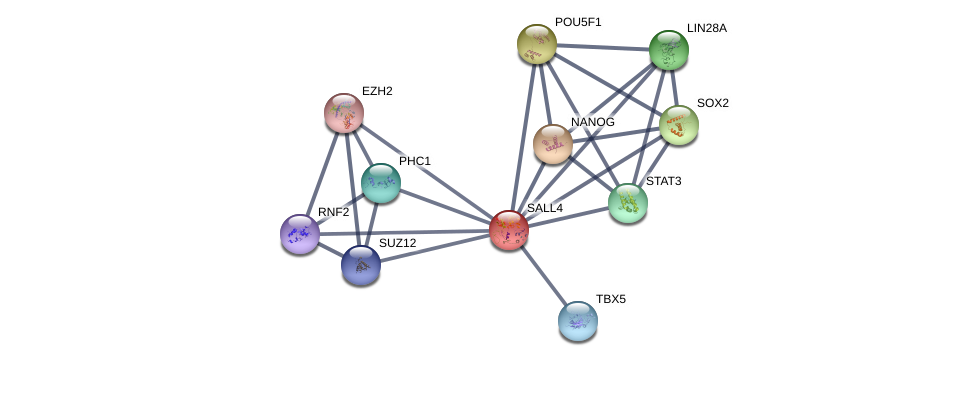
\includegraphics[width=\textwidth,height=0.7\textheight]{images/talk06/string_normal_image.png}
\caption{interacting partners of SALL4}
\end{figure}
\end{frame}

\begin{frame}{note to previous plot}
\protect\hypertarget{note-to-previous-plot}{}
\textbf{note} this plot was generated using the following parameters:

\begin{itemize}
\tightlist
\item
  use SALL4 in human as query
\item
  show only the top ten connectivity partners
\item
  only connectivity score \textgreater= 900 (or 0.9) were shown
\end{itemize}
\end{frame}

\begin{frame}{tasks of task 1}
\protect\hypertarget{tasks-of-task-1}{}
\begin{enumerate}
\tightlist
\item
  get human PPI data
\item
  limit the interactions to those with scores \textgreater= 900 (or 0.9)
\item
  find SALL4 and its top ten interaction parteners
\item
  visualize the PPI network
\item
  calculate connectivities of sall4 and its top ten parteners in the
  dataset
\end{enumerate}

\textbf{问题}

生物学意义何在??
\end{frame}

\begin{frame}{download human ppi data from STRING}
\protect\hypertarget{download-human-ppi-data-from-string}{}
go to : \url{https://string-db.org/cgi/download.pl}

\begin{figure}
\centering
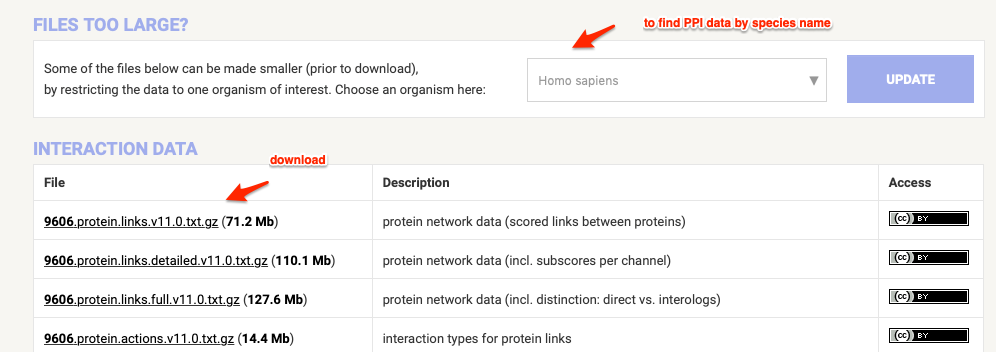
\includegraphics[width=\textwidth,height=0.5\textheight]{images/talk06/download_human_PPI_from_string.png}
\caption{Download human PPI data from STRING}
\end{figure}
\end{frame}

\begin{frame}[fragile]{load and load the human PPI data}
\protect\hypertarget{load-and-load-the-human-ppi-data}{}
\FontSmall

\begin{Shaded}
\begin{Highlighting}[]
\FunctionTok{library}\NormalTok{(tidyverse);}
\end{Highlighting}
\end{Shaded}

\begin{Shaded}
\begin{Highlighting}[]
\DocumentationTok{\#\# read\_csv 也能处理压缩文件!!! }
\NormalTok{ppi }\OtherTok{\textless{}{-}} \FunctionTok{read\_delim}\NormalTok{( }\AttributeTok{file =} \StringTok{"data/talk06/ppi900.txt.gz"}\NormalTok{, }\AttributeTok{col\_names =}\NormalTok{ T, }
                   \AttributeTok{delim =}  \StringTok{"}\SpecialCharTok{\textbackslash{}t}\StringTok{"}\NormalTok{, }\AttributeTok{quote =} \StringTok{""}\NormalTok{ );}

\DocumentationTok{\#\# 查看一下数据 {-}{-}}
\NormalTok{ppi }\SpecialCharTok{\%\textgreater{}\%} \FunctionTok{filter}\NormalTok{( gene1 }\SpecialCharTok{==} \StringTok{"SALL4"}\NormalTok{ ) }\SpecialCharTok{\%\textgreater{}\%} \FunctionTok{do}\NormalTok{( }\FunctionTok{head}\NormalTok{(.,  }\AttributeTok{n =} \DecValTok{10}\NormalTok{ ) );}
\end{Highlighting}
\end{Shaded}

\begin{verbatim}
## # A tibble: 10 x 3
##    gene1 gene2   score
##    <chr> <chr>   <dbl>
##  1 SALL4 POLR2E    900
##  2 SALL4 POLR2C    900
##  3 SALL4 POLR2I    900
##  4 SALL4 NANOG     992
##  5 SALL4 SALL1     923
##  6 SALL4 ZSCAN10   912
##  7 SALL4 LIN28A    957
##  8 SALL4 POU5F1    986
##  9 SALL4 SMAD2     906
## 10 SALL4 EPAS1     900
\end{verbatim}
\end{frame}

\begin{frame}[fragile]{start to process the data}
\protect\hypertarget{start-to-process-the-data}{}
\FontSmall

\begin{Shaded}
\begin{Highlighting}[]
\DocumentationTok{\#\# get top 10 interacting partners of SALL4 by interaction score ... }
\NormalTok{toppart }\OtherTok{\textless{}{-}}\NormalTok{ ppi }\SpecialCharTok{\%\textgreater{}\%} \FunctionTok{filter}\NormalTok{( gene1 }\SpecialCharTok{==} \StringTok{"SALL4"}\NormalTok{ ) }\SpecialCharTok{\%\textgreater{}\%} 
  \FunctionTok{arrange}\NormalTok{( }\FunctionTok{desc}\NormalTok{( score ) ) }\SpecialCharTok{\%\textgreater{}\%} \FunctionTok{slice}\NormalTok{( }\DecValTok{1}\SpecialCharTok{:}\DecValTok{10}\NormalTok{ );}

\DocumentationTok{\#\# get the interaction network consisting the top genes {-}{-}}
\NormalTok{genes }\OtherTok{\textless{}{-}} \FunctionTok{unique}\NormalTok{( }\FunctionTok{c}\NormalTok{( }\StringTok{"SALL4"}\NormalTok{, toppart}\SpecialCharTok{$}\NormalTok{gene2 ) );}
\NormalTok{netdata }\OtherTok{\textless{}{-}}\NormalTok{ ppi }\SpecialCharTok{\%\textgreater{}\%} \FunctionTok{filter}\NormalTok{( gene1 }\SpecialCharTok{\%in\%}\NormalTok{ genes }\SpecialCharTok{\&}\NormalTok{ gene2 }\SpecialCharTok{\%in\%}\NormalTok{ genes );}
\FunctionTok{nrow}\NormalTok{(netdata);}
\end{Highlighting}
\end{Shaded}

\begin{verbatim}
## [1] 80
\end{verbatim}
\end{frame}

\begin{frame}[fragile]{load the igraph package}
\protect\hypertarget{load-the-igraph-package}{}
\FontSmall

\begin{Shaded}
\begin{Highlighting}[]
\DocumentationTok{\#\# {-}{-} to make sure the installation will only run once ... }
\ControlFlowTok{if}\NormalTok{ (}\SpecialCharTok{!}\FunctionTok{require}\NormalTok{(}\StringTok{"igraph"}\NormalTok{))\{ }
  \FunctionTok{chooseCRANmirror}\NormalTok{();}
  \FunctionTok{install.packages}\NormalTok{(}\StringTok{"igraph"}\NormalTok{);}
\NormalTok{\} }

\FunctionTok{library}\NormalTok{( igraph );}
\end{Highlighting}
\end{Shaded}
\end{frame}

\begin{frame}[fragile]{visualise the network \ldots{}}
\protect\hypertarget{visualise-the-network}{}
\FontSmall

\begin{Shaded}
\begin{Highlighting}[]
\NormalTok{netnet }\OtherTok{\textless{}{-}} \FunctionTok{graph\_from\_data\_frame}\NormalTok{( netdata, }\AttributeTok{directed =} \ConstantTok{FALSE}\NormalTok{ );}
\FunctionTok{plot}\NormalTok{(netnet);}
\end{Highlighting}
\end{Shaded}

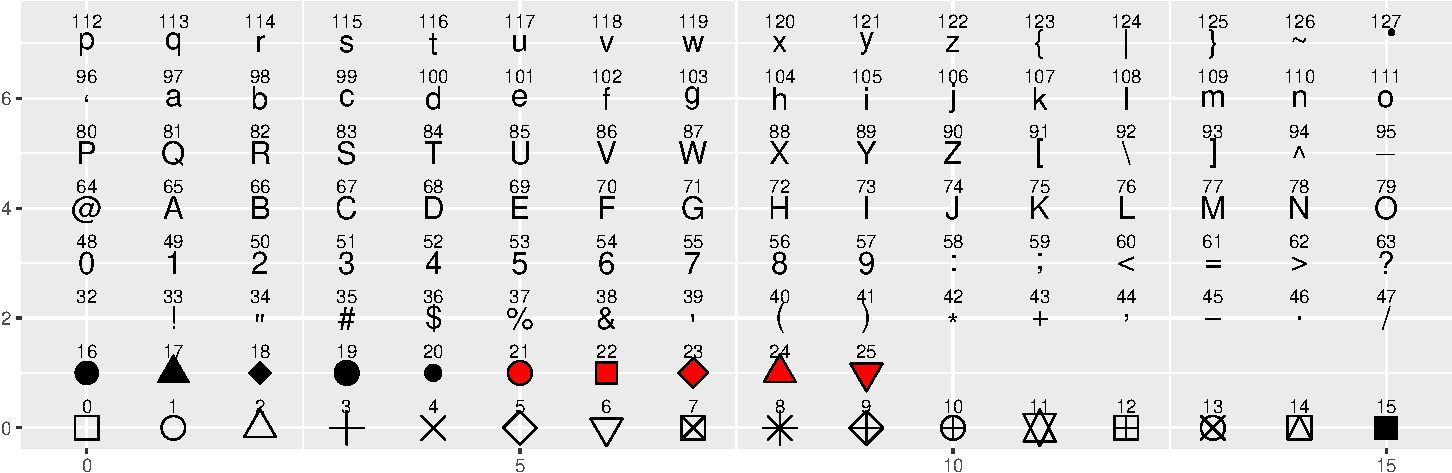
\includegraphics{/Users/lucas/Library/Mobile Documents/com~apple~CloudDocs/~~aa学习/大二上/学习/R for Data Science/R-for-Data-Science/talk06-practices_files/figure-beamer/unnamed-chunk-6-1.pdf}
\end{frame}

\begin{frame}{图的问题}
\protect\hypertarget{ux56feux7684ux95eeux9898}{}
\begin{itemize}
\tightlist
\item
  very ugly
\item
  two lines (redundancy) between every two nodes
\end{itemize}
\end{frame}

\begin{frame}[fragile]{redundancy among data}
\protect\hypertarget{redundancy-among-data}{}
\FontSmall

\begin{Shaded}
\begin{Highlighting}[]
\NormalTok{netdata }\SpecialCharTok{\%\textgreater{}\%} \FunctionTok{filter}\NormalTok{( gene1 }\SpecialCharTok{\%in\%} \FunctionTok{c}\NormalTok{(}\StringTok{"SALL4"}\NormalTok{, }\StringTok{"NANOG"}\NormalTok{) }\SpecialCharTok{\&}\NormalTok{ gene2 }\SpecialCharTok{\%in\%} \FunctionTok{c}\NormalTok{(}\StringTok{"SALL4"}\NormalTok{, }\StringTok{"NANOG"}\NormalTok{) );}
\end{Highlighting}
\end{Shaded}

\begin{verbatim}
## # A tibble: 2 x 3
##   gene1 gene2 score
##   <chr> <chr> <dbl>
## 1 NANOG SALL4   992
## 2 SALL4 NANOG   992
\end{verbatim}
\end{frame}

\begin{frame}[fragile]{how to remove redundancy?}
\protect\hypertarget{how-to-remove-redundancy}{}
\FontSmall

\begin{Shaded}
\begin{Highlighting}[]
\DocumentationTok{\#\# create a new column, sort the two gene names, and concatenate them ... }
\NormalTok{testdata }\OtherTok{\textless{}{-}} 
\NormalTok{  netdata }\SpecialCharTok{\%\textgreater{}\%} \FunctionTok{filter}\NormalTok{( gene1 }\SpecialCharTok{\%in\%} \FunctionTok{c}\NormalTok{(}\StringTok{"SALL4"}\NormalTok{, }\StringTok{"NANOG"}\NormalTok{) }\SpecialCharTok{\&}\NormalTok{ gene2 }\SpecialCharTok{\%in\%} \FunctionTok{c}\NormalTok{(}\StringTok{"SALL4"}\NormalTok{, }\StringTok{"NANOG"}\NormalTok{) ) }\SpecialCharTok{\%\textgreater{}\%} 
  \FunctionTok{mutate}\NormalTok{( }\AttributeTok{group  =}  
            \FunctionTok{if\_else}\NormalTok{( gene1 }\SpecialCharTok{\textgreater{}}\NormalTok{ gene2, }
                     \FunctionTok{str\_c}\NormalTok{( gene1, gene2, }\AttributeTok{sep =} \StringTok{"{-}"}\NormalTok{ ), }
                     \FunctionTok{str\_c}\NormalTok{( gene2, gene1, }\AttributeTok{sep =} \StringTok{"{-}"}\NormalTok{ ) ) );}

\NormalTok{testdata;}
\end{Highlighting}
\end{Shaded}

\begin{verbatim}
## # A tibble: 2 x 4
##   gene1 gene2 score group      
##   <chr> <chr> <dbl> <chr>      
## 1 NANOG SALL4   992 SALL4-NANOG
## 2 SALL4 NANOG   992 SALL4-NANOG
\end{verbatim}

\FontNormal

\textbf{Note} \texttt{str\_c} is from the \texttt{stringr} package!!
\end{frame}

\begin{frame}[fragile]{remove redundancy!}
\protect\hypertarget{remove-redundancy}{}
\FontSmall

\begin{Shaded}
\begin{Highlighting}[]
\NormalTok{testdata }\SpecialCharTok{\%\textgreater{}\%} \FunctionTok{group\_by}\NormalTok{( group ) }\SpecialCharTok{\%\textgreater{}\%} \FunctionTok{slice}\NormalTok{( }\DecValTok{1}\NormalTok{ );}
\end{Highlighting}
\end{Shaded}

\begin{verbatim}
## # A tibble: 1 x 4
## # Groups:   group [1]
##   gene1 gene2 score group      
##   <chr> <chr> <dbl> <chr>      
## 1 NANOG SALL4   992 SALL4-NANOG
\end{verbatim}
\end{frame}

\begin{frame}[fragile]{remove redundancy, cont.}
\protect\hypertarget{remove-redundancy-cont.}{}
\FontSmall

\begin{Shaded}
\begin{Highlighting}[]
\NormalTok{netdata.nr }\OtherTok{\textless{}{-}} 
\NormalTok{  netdata }\SpecialCharTok{\%\textgreater{}\%} 
  \FunctionTok{mutate}\NormalTok{( }\AttributeTok{group  =}  
            \FunctionTok{if\_else}\NormalTok{( gene1 }\SpecialCharTok{\textgreater{}}\NormalTok{ gene2, }
                     \FunctionTok{str\_c}\NormalTok{( gene1, gene2, }\AttributeTok{sep =} \StringTok{"{-}"}\NormalTok{ ), }
                     \FunctionTok{str\_c}\NormalTok{( gene2, gene1, }\AttributeTok{sep =} \StringTok{"{-}"}\NormalTok{ ) ) ) }\SpecialCharTok{\%\textgreater{}\%} 
  \FunctionTok{group\_by}\NormalTok{( group ) }\SpecialCharTok{\%\textgreater{}\%} \FunctionTok{slice}\NormalTok{( }\DecValTok{1}\NormalTok{ );}

\FunctionTok{nrow}\NormalTok{(netdata.nr);}
\end{Highlighting}
\end{Shaded}

\begin{verbatim}
## [1] 40
\end{verbatim}
\end{frame}

\begin{frame}[fragile]{plot the non-redundant data}
\protect\hypertarget{plot-the-non-redundant-data}{}
\FontSmall

\begin{Shaded}
\begin{Highlighting}[]
\NormalTok{netnet.nr }\OtherTok{\textless{}{-}} \FunctionTok{graph\_from\_data\_frame}\NormalTok{( netdata.nr, }\AttributeTok{directed =} \ConstantTok{FALSE}\NormalTok{ );}
\FunctionTok{plot}\NormalTok{(netnet.nr);}
\end{Highlighting}
\end{Shaded}

\includegraphics{/Users/lucas/Library/Mobile Documents/com~apple~CloudDocs/~~aa学习/大二上/学习/R for Data Science/R-for-Data-Science/talk06-practices_files/figure-beamer/unnamed-chunk-11-1.pdf}
\end{frame}

\begin{frame}[fragile]{redundant 的数据可以用来计算 degree}
\protect\hypertarget{redundant-ux7684ux6570ux636eux53efux4ee5ux7528ux6765ux8ba1ux7b97-degree}{}
\FontSmall

\begin{Shaded}
\begin{Highlighting}[]
\NormalTok{net.stats }\OtherTok{\textless{}{-}} 
\NormalTok{  netdata }\SpecialCharTok{\%\textgreater{}\%} \FunctionTok{group\_by}\NormalTok{( gene1 ) }\SpecialCharTok{\%\textgreater{}\%} \FunctionTok{summarise}\NormalTok{( }\AttributeTok{degree =} \FunctionTok{n}\NormalTok{() ) }\SpecialCharTok{\%\textgreater{}\%} 
  \FunctionTok{arrange}\NormalTok{( }\FunctionTok{desc}\NormalTok{ (degree) );}
\NormalTok{net.stats;}
\end{Highlighting}
\end{Shaded}

\begin{verbatim}
## # A tibble: 11 x 2
##    gene1   degree
##    <chr>    <int>
##  1 SALL4       10
##  2 SOX2        10
##  3 NANOG        9
##  4 POU5F1       9
##  5 KLF4         8
##  6 LIN28A       8
##  7 PRDM14       7
##  8 ZSCAN10      7
##  9 STAT3        5
## 10 SALL1        4
## 11 CTNNB1       3
\end{verbatim}
\end{frame}

\begin{frame}[fragile]{继续美化 network}
\protect\hypertarget{ux7ee7ux7eedux7f8eux5316-network}{}
\FontSmall

\begin{Shaded}
\begin{Highlighting}[]
\DocumentationTok{\#\# node大小由degree决定}
\DocumentationTok{\#\# 查看网络中基因名存储的顺序}
\FunctionTok{V}\NormalTok{(netnet.nr)}\SpecialCharTok{$}\NormalTok{name; }
\end{Highlighting}
\end{Shaded}

\begin{verbatim}
##  [1] "KLF4"    "LIN28A"  "POU5F1"  "PRDM14"  "SALL1"   "CTNNB1"  "NANOG"  
##  [8] "SOX2"    "STAT3"   "ZSCAN10" "SALL4"
\end{verbatim}

\begin{Shaded}
\begin{Highlighting}[]
\DocumentationTok{\#\# 获取它们相对应的 degree ...}
\NormalTok{net.stats[}\FunctionTok{match}\NormalTok{( }\FunctionTok{V}\NormalTok{(netnet.nr)}\SpecialCharTok{$}\NormalTok{name , net.stats}\SpecialCharTok{$}\NormalTok{gene1 ),  ];}
\end{Highlighting}
\end{Shaded}

\begin{verbatim}
## # A tibble: 11 x 2
##    gene1   degree
##    <chr>    <int>
##  1 KLF4         8
##  2 LIN28A       8
##  3 POU5F1       9
##  4 PRDM14       7
##  5 SALL1        4
##  6 CTNNB1       3
##  7 NANOG        9
##  8 SOX2        10
##  9 STAT3        5
## 10 ZSCAN10      7
## 11 SALL4       10
\end{verbatim}
\end{frame}

\begin{frame}[fragile]{继续美化 network, cont.}
\protect\hypertarget{ux7ee7ux7eedux7f8eux5316-network-cont.}{}
\FontSmall

\begin{Shaded}
\begin{Highlighting}[]
\FunctionTok{vertex\_attr}\NormalTok{(netnet.nr, }\StringTok{"size"}\NormalTok{) }\OtherTok{\textless{}{-}} 
\NormalTok{  net.stats}\SpecialCharTok{$}\NormalTok{degree[}\FunctionTok{match}\NormalTok{( }\FunctionTok{V}\NormalTok{(netnet.nr)}\SpecialCharTok{$}\NormalTok{name , net.stats}\SpecialCharTok{$}\NormalTok{gene1 ) ] }\SpecialCharTok{*} \DecValTok{2}\NormalTok{;}
\FunctionTok{plot}\NormalTok{( netnet.nr );}
\end{Highlighting}
\end{Shaded}

\includegraphics{/Users/lucas/Library/Mobile Documents/com~apple~CloudDocs/~~aa学习/大二上/学习/R for Data Science/R-for-Data-Science/talk06-practices_files/figure-beamer/unnamed-chunk-14-1.pdf}
\end{frame}

\begin{frame}{更多美化}
\protect\hypertarget{ux66f4ux591aux7f8eux5316}{}
详见:

\begin{enumerate}
\tightlist
\item
  igraph introduction
\item
  a comprehensive network visualization tutorial in R
\end{enumerate}

\begin{figure}
\centering
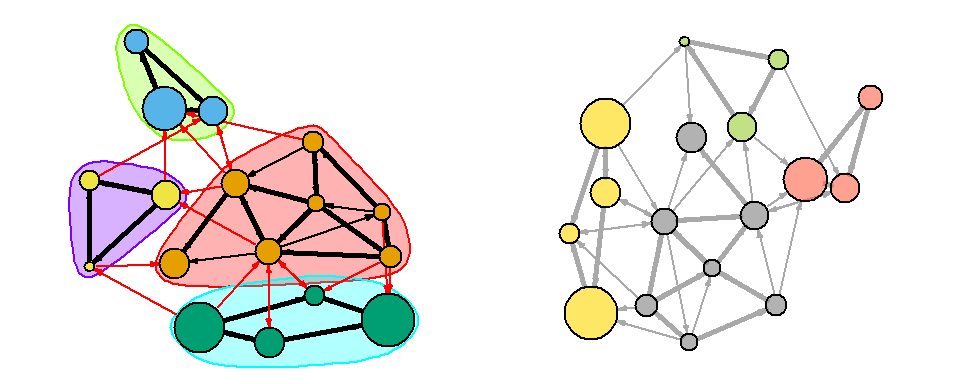
\includegraphics[width=\textwidth,height=0.4\textheight]{images/talk06/igraph_example.png}
\caption{Example final outcomes}
\end{figure}
\end{frame}

\begin{frame}[fragile]{other network visualisation packages}
\protect\hypertarget{other-network-visualisation-packages}{}
\begin{enumerate}
\tightlist
\item
  \texttt{ggnet}
\item
  \texttt{interactive\ networkD3\ R\ package}
\item
  \texttt{plotly.js}
\item
  \texttt{D3}
\end{enumerate}
\end{frame}

\begin{frame}{生信任务2 : 宏基因基因数据展示的小应用 (forcats)}
\protect\hypertarget{ux751fux4fe1ux4efbux52a12-ux5b8fux57faux56e0ux57faux56e0ux6570ux636eux5c55ux793aux7684ux5c0fux5e94ux7528-forcats}{}
\begin{figure}
\centering
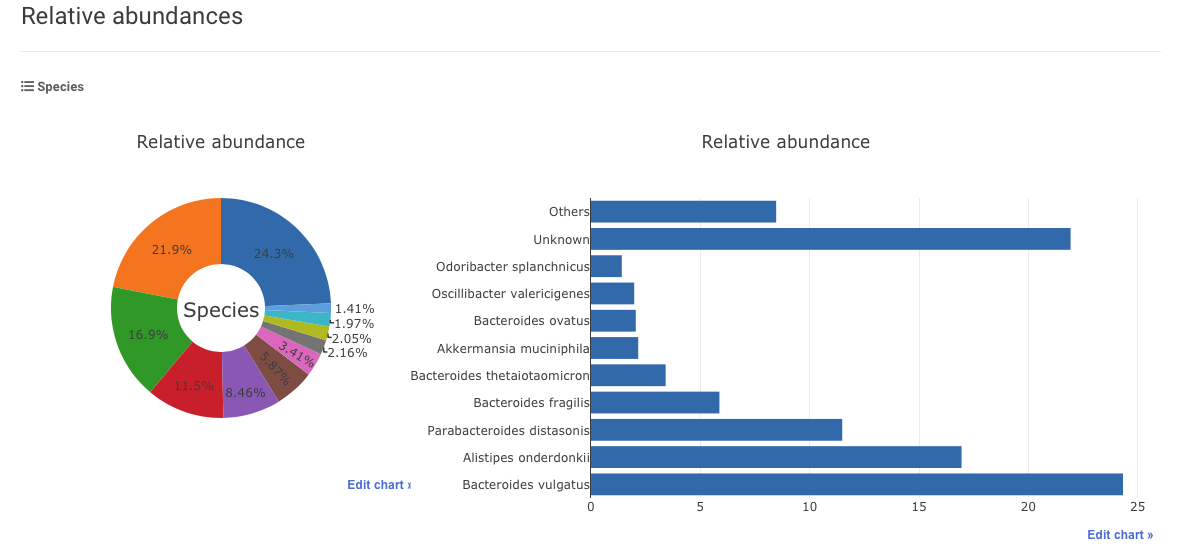
\includegraphics[width=\textwidth,height=0.6\textheight]{images/talk06/gmrepo_run_statistics.png}
\caption{肠道物种丰度示意图}
\end{figure}

Find more at the \href{https://gmrepo.humangut.info/home}{GMrepo
database}.
\end{frame}

\begin{frame}{什么是宏基因组?}
\protect\hypertarget{ux4ec0ux4e48ux662fux5b8fux57faux56e0ux7ec4}{}
Metagenomics is the study of genetic material recovered directly from
environmental samples.

\begin{block}{research contents}
\protect\hypertarget{research-contents}{}
\begin{itemize}
\tightlist
\item
  mostly prokaryotes
\item
  unicellular eukaryotes
\item
  viruses
\end{itemize}
\end{block}

\begin{block}{techniques}
\protect\hypertarget{techniques}{}
\begin{itemize}
\tightlist
\item
  16S (universially conserved gene in prokaryotes)
\item
  whole genome sequencing (WGS or metagenomics)
\end{itemize}
\end{block}
\end{frame}

\begin{frame}{what can metagenomics do?}
\protect\hypertarget{what-can-metagenomics-do}{}
\begin{itemize}
\tightlist
\item
  identify new species
\item
  reveal species kinds and abundances
\item
  relate species changes to human health and disease
\end{itemize}
\end{frame}

\begin{frame}[fragile]{biomes}
\protect\hypertarget{biomes}{}
\begin{figure}
\centering
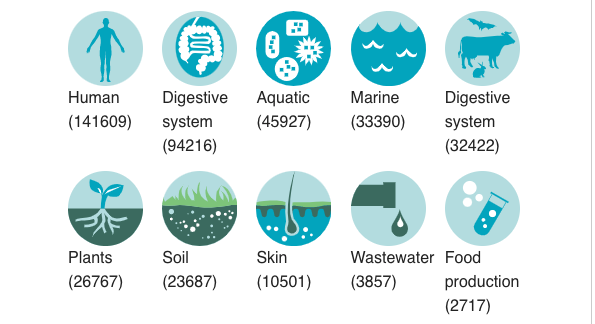
\includegraphics[width=\textwidth,height=0.6\textheight]{images/talk06/ebi_metagenomics_biomes_aug4_2021.png}
\caption{Biomes}
\end{figure}

Screenshot taken from the \texttt{EBI\ MGnify\ database} on
\texttt{Aug\ 4,\ 2021};
\end{frame}

\begin{frame}{enviromental microbiome}
\protect\hypertarget{enviromental-microbiome}{}
\begin{itemize}
\tightlist
\item
  soil
\item
  ocean
\end{itemize}

\begin{figure}
\centering
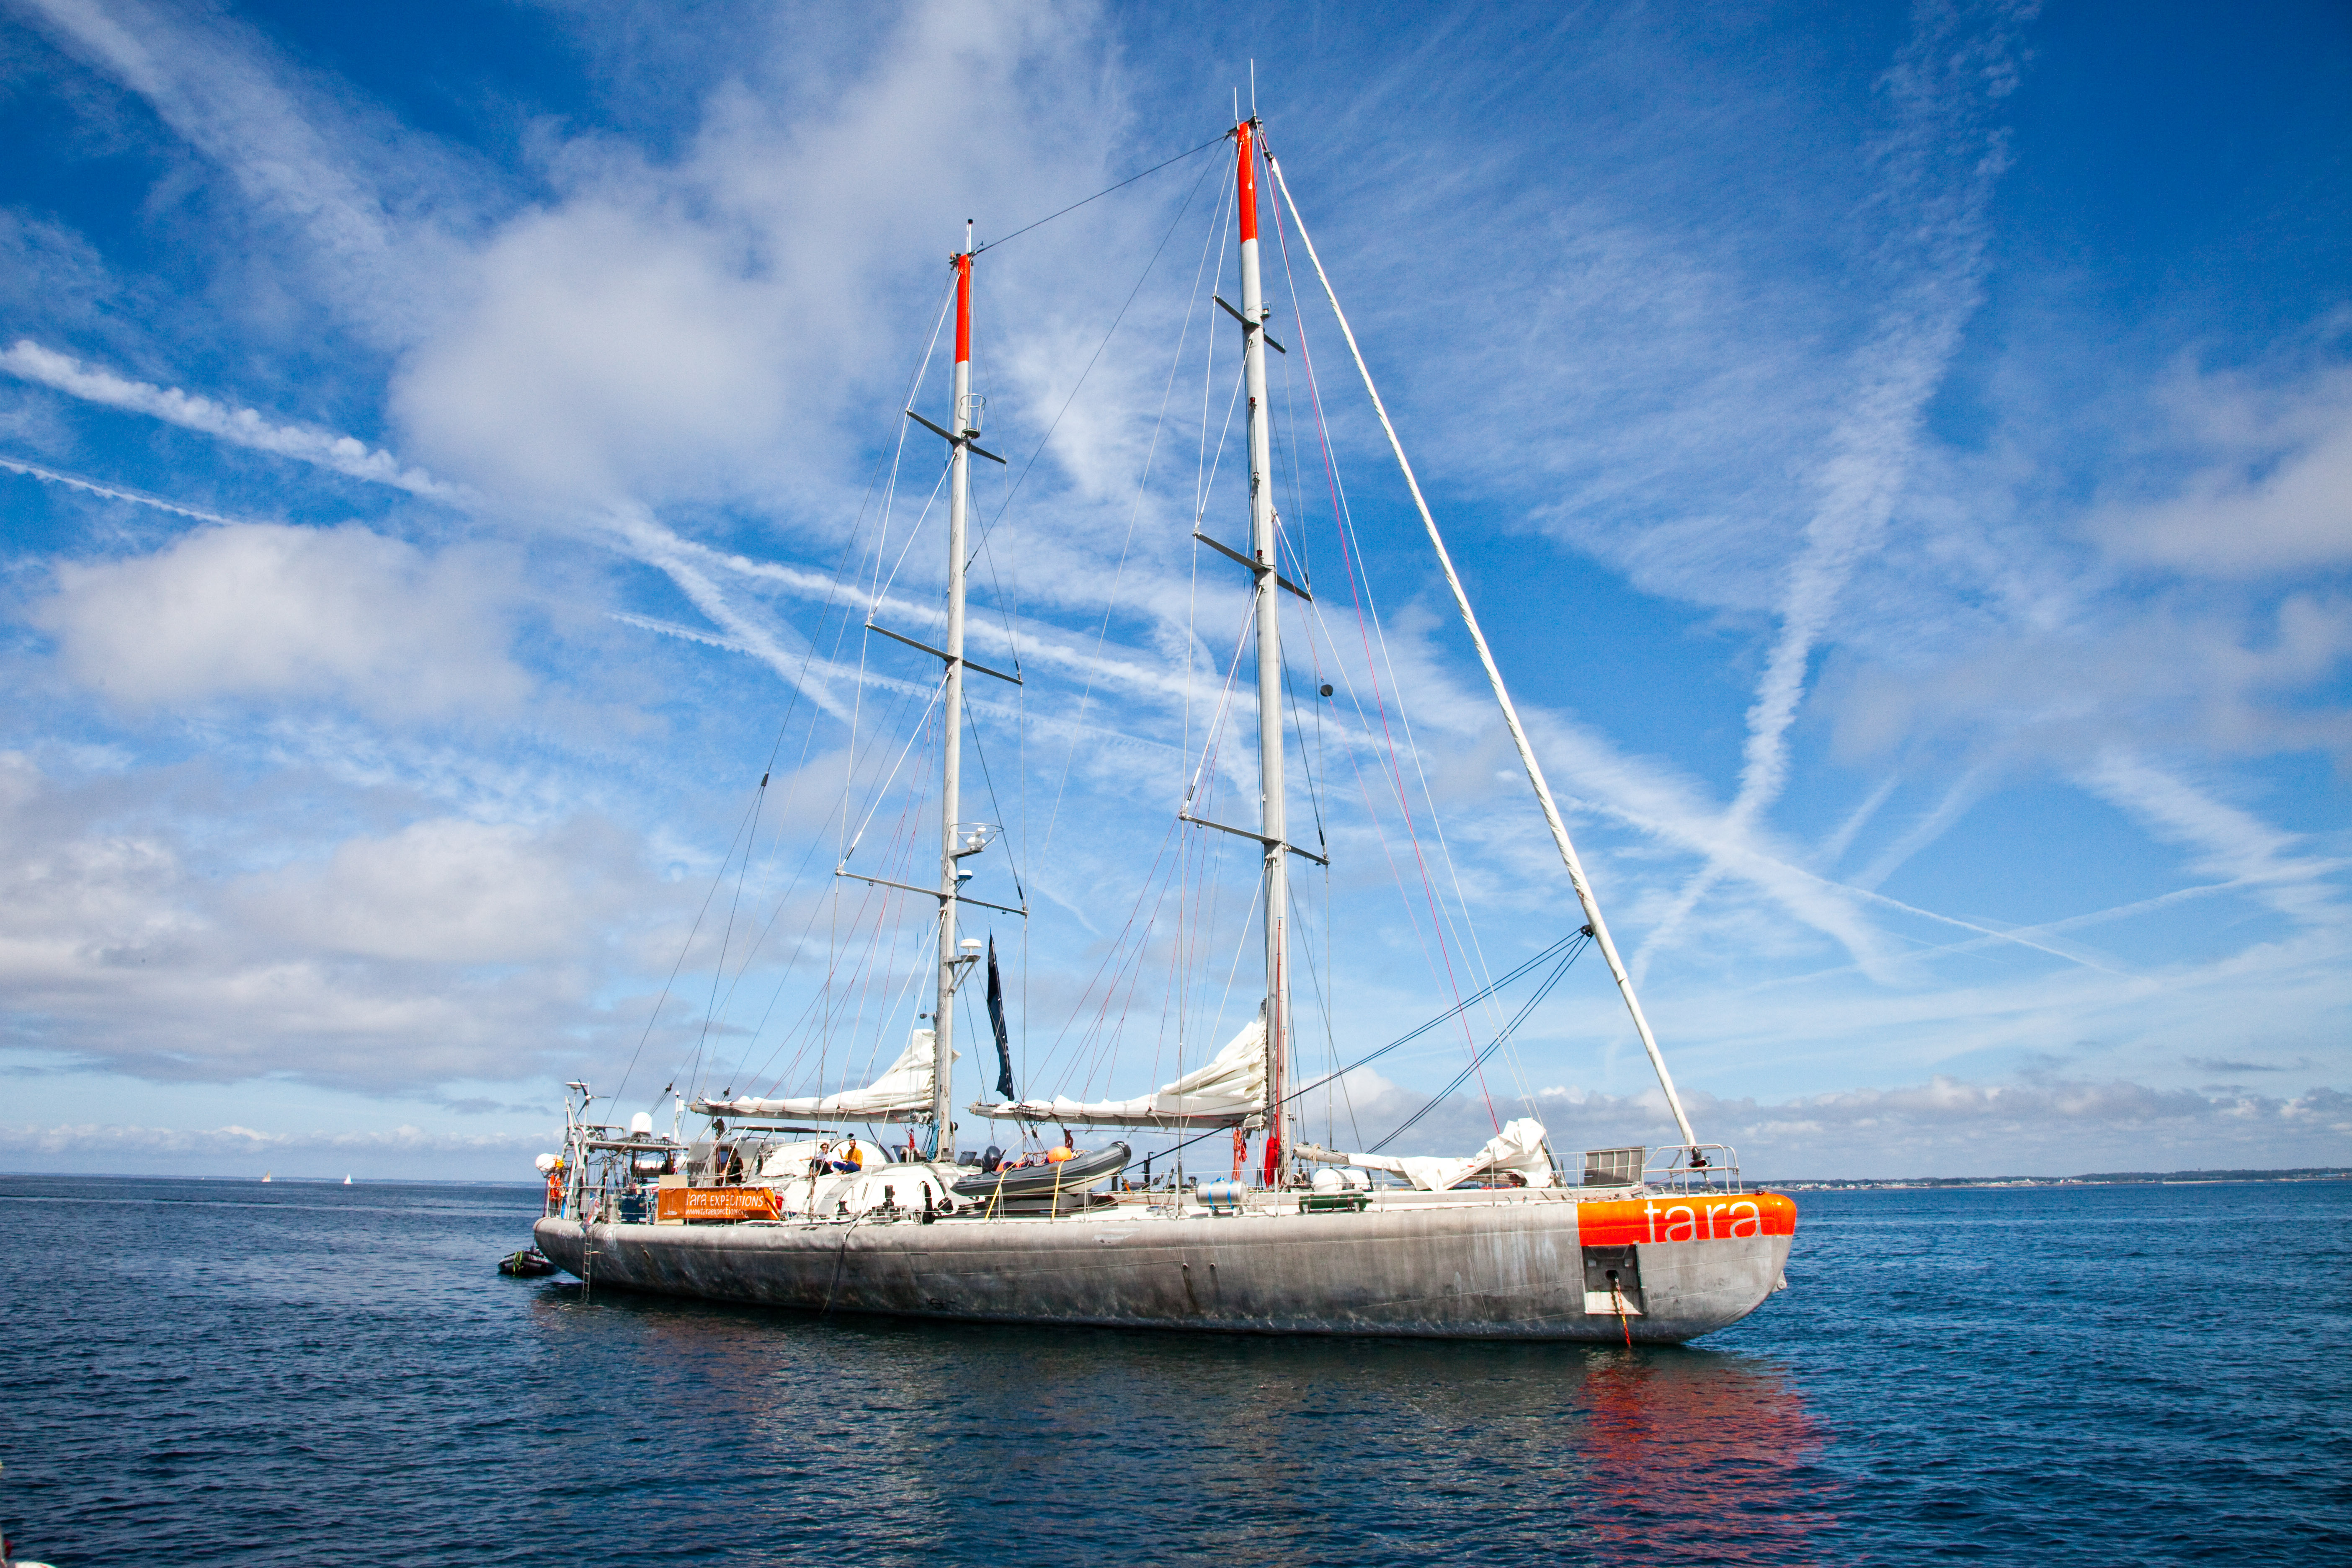
\includegraphics[width=\textwidth,height=0.5\textheight]{images/talk06/tara_oceans_boat.jpg}
\caption{The tara oceans expedition}
\end{figure}
\end{frame}

\begin{frame}{host associated microbiomes}
\protect\hypertarget{host-associated-microbiomes}{}
\begin{itemize}
\tightlist
\item
  human body sites
\item
  animals \& plants
\end{itemize}

\begin{figure}
\centering

\includegraphics[width=\textwidth,height=0.3\textheight]{images/talk06/iHMP.png}
\caption{NIH human microbiome project}
\end{figure}
\end{frame}

\begin{frame}{why human gut microbiota is important?}
\protect\hypertarget{why-human-gut-microbiota-is-important}{}
\begin{figure}
\centering
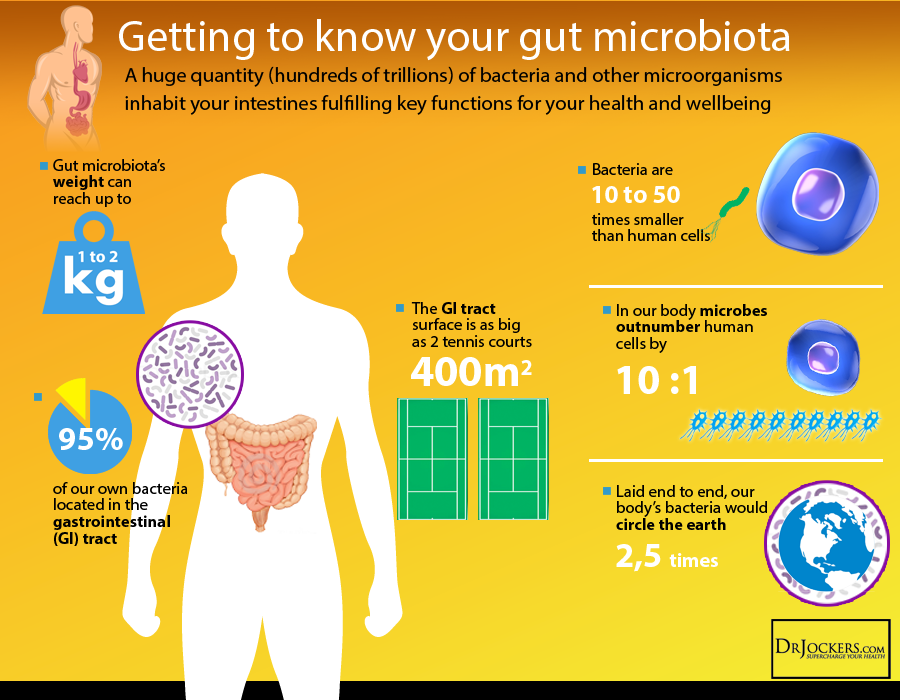
\includegraphics[width=\textwidth,height=0.6\textheight]{images/talk06/GutMicrobeInfographic.png}
\caption{human gut microbita}
\end{figure}
\end{frame}

\begin{frame}{tasks of human gut microbiota analysis}
\protect\hypertarget{tasks-of-human-gut-microbiota-analysis}{}
\begin{itemize}
\tightlist
\item
  identify new species
\item
  find good, bad and commensal microbes
\item
  link microbial variations to human health
\item
  mechanisms
\item
  modulation, intervention and regulation
\end{itemize}
\end{frame}

\begin{frame}[fragile]{typical human gut microbiome data}
\protect\hypertarget{typical-human-gut-microbiome-data}{}
Species abundances

\FontSmall

\begin{Shaded}
\begin{Highlighting}[]
\NormalTok{abu }\OtherTok{\textless{}{-}} 
  \FunctionTok{read\_delim}\NormalTok{(}
    \AttributeTok{file =} \StringTok{"data/talk06/relative\_abundance\_for\_RUN\_ERR1072629\_taxonlevel\_species.txt"}\NormalTok{,}
    \AttributeTok{delim =} \StringTok{"}\SpecialCharTok{\textbackslash{}t}\StringTok{"}\NormalTok{, }\AttributeTok{quote =} \StringTok{""}\NormalTok{, }\AttributeTok{comment =} \StringTok{"\#"}\NormalTok{);}
\end{Highlighting}
\end{Shaded}

\begin{verbatim}
## Rows: 122 Columns: 3
## -- Column specification --------------------------------------------------------
## Delimiter: "\t"
## chr (1): scientific_name
## dbl (2): ncbi_taxon_id, relative_abundance
## 
## i Use `spec()` to retrieve the full column specification for this data.
## i Specify the column types or set `show_col_types = FALSE` to quiet this message.
\end{verbatim}

\begin{Shaded}
\begin{Highlighting}[]
\FunctionTok{nrow}\NormalTok{(abu);}
\end{Highlighting}
\end{Shaded}

\begin{verbatim}
## [1] 122
\end{verbatim}
\end{frame}

\begin{frame}[fragile]{Species abundances, cont.}
\protect\hypertarget{species-abundances-cont.}{}
\FontSmall

\begin{Shaded}
\begin{Highlighting}[]
\NormalTok{abu }\SpecialCharTok{\%\textgreater{}\%} \FunctionTok{arrange}\NormalTok{( }\FunctionTok{desc}\NormalTok{( relative\_abundance ) ) }\SpecialCharTok{\%\textgreater{}\%} \FunctionTok{do}\NormalTok{( }\FunctionTok{head}\NormalTok{(., }\AttributeTok{n =} \DecValTok{10}\NormalTok{) );}
\end{Highlighting}
\end{Shaded}

\begin{verbatim}
## # A tibble: 10 x 3
##    ncbi_taxon_id relative_abundance scientific_name             
##            <dbl>              <dbl> <chr>                       
##  1           821              24.3  Bacteroides vulgatus        
##  2            -1              21.9  Unknown                     
##  3        328813              16.9  Alistipes onderdonkii       
##  4           823              11.5  Parabacteroides distasonis  
##  5           817               5.87 Bacteroides fragilis        
##  6           818               3.41 Bacteroides thetaiotaomicron
##  7        239935               2.16 Akkermansia muciniphila     
##  8         28116               2.05 Bacteroides ovatus          
##  9        351091               1.97 Oscillibacter valericigenes 
## 10         28118               1.41 Odoribacter splanchnicus
\end{verbatim}
\end{frame}

\begin{frame}{相对丰度作图要求}
\protect\hypertarget{ux76f8ux5bf9ux4e30ux5ea6ux4f5cux56feux8981ux6c42}{}
\begin{enumerate}
\tightlist
\item
  按丰度从高到低排序
\item
  只取前10个species (保留10行)
\item
  将后面的丰度累加在一起,汇总为''Others''分类
\end{enumerate}
\end{frame}

\begin{frame}[fragile]{数据处理}
\protect\hypertarget{ux6570ux636eux5904ux7406}{}
\FontSmall

\begin{Shaded}
\begin{Highlighting}[]
\FunctionTok{library}\NormalTok{( tidytidbits );}
\NormalTok{abu.dat }\OtherTok{\textless{}{-}} 
\NormalTok{  abu }\SpecialCharTok{\%\textgreater{}\%} \FunctionTok{arrange}\NormalTok{( }\FunctionTok{desc}\NormalTok{( relative\_abundance ) ) }\SpecialCharTok{\%\textgreater{}\%} 
    \FunctionTok{lump\_rows}\NormalTok{( scientific\_name, relative\_abundance, }\AttributeTok{n =} \DecValTok{10}\NormalTok{, }\AttributeTok{other\_level =} \StringTok{"Others"}\NormalTok{ );}

\FunctionTok{head}\NormalTok{(abu.dat, }\AttributeTok{n =} \DecValTok{11}\NormalTok{);}
\end{Highlighting}
\end{Shaded}

\begin{verbatim}
## # A tibble: 11 x 3
##    ncbi_taxon_id relative_abundance scientific_name             
##            <dbl>              <dbl> <chr>                       
##  1           821              24.3  Bacteroides vulgatus        
##  2            -1              21.9  Unknown                     
##  3        328813              16.9  Alistipes onderdonkii       
##  4           823              11.5  Parabacteroides distasonis  
##  5           817               5.87 Bacteroides fragilis        
##  6           818               3.41 Bacteroides thetaiotaomicron
##  7        239935               2.16 Akkermansia muciniphila     
##  8         28116               2.05 Bacteroides ovatus          
##  9        351091               1.97 Oscillibacter valericigenes 
## 10         28118               1.41 Odoribacter splanchnicus    
## 11      31199992               8.46 Others
\end{verbatim}
\end{frame}

\begin{frame}[fragile]{尝试作图}
\protect\hypertarget{ux5c1dux8bd5ux4f5cux56fe}{}
\FontSmall

\begin{Shaded}
\begin{Highlighting}[]
\FunctionTok{ggplot}\NormalTok{(abu.dat, }\FunctionTok{aes}\NormalTok{(}\AttributeTok{x =}\NormalTok{ scientific\_name, }\AttributeTok{y =}\NormalTok{ relative\_abundance, }\AttributeTok{fill =}\NormalTok{ scientific\_name ) ) }\SpecialCharTok{+} 
  \FunctionTok{geom\_bar}\NormalTok{( }\AttributeTok{stat =} \StringTok{"identity"}\NormalTok{ ) }\SpecialCharTok{+} 
  \FunctionTok{coord\_flip}\NormalTok{()}
\end{Highlighting}
\end{Shaded}

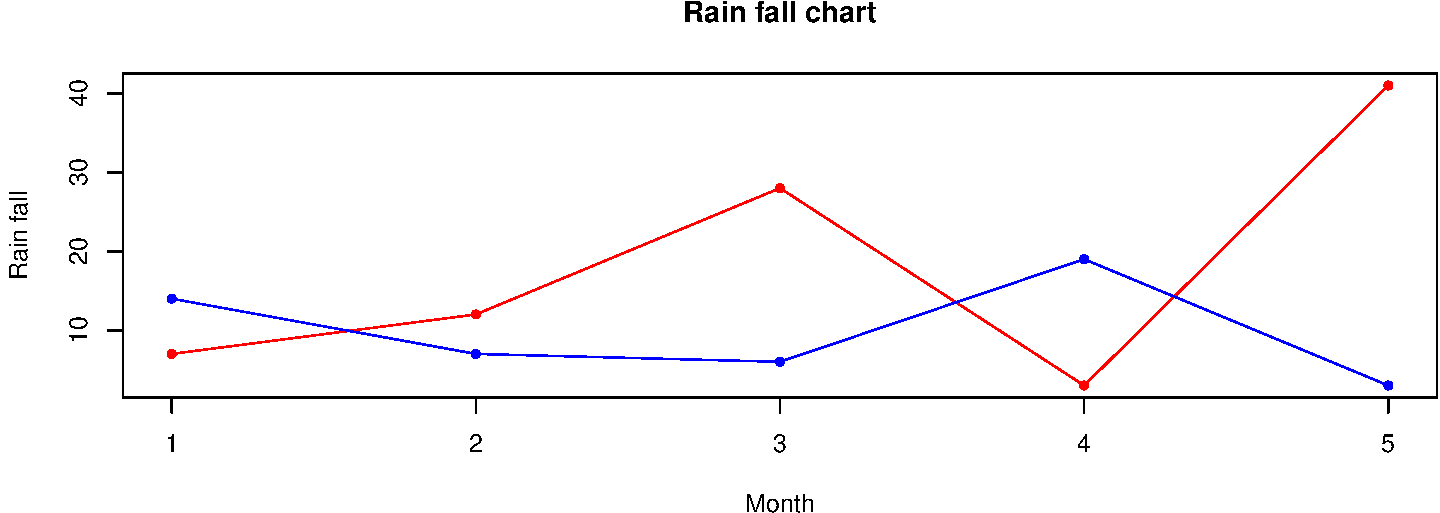
\includegraphics{/Users/lucas/Library/Mobile Documents/com~apple~CloudDocs/~~aa学习/大二上/学习/R for Data Science/R-for-Data-Science/talk06-practices_files/figure-beamer/unnamed-chunk-18-1.pdf}
\end{frame}

\begin{frame}[fragile]{调整排列顺序}
\protect\hypertarget{ux8c03ux6574ux6392ux5217ux987aux5e8f}{}
\FontSmall

\begin{Shaded}
\begin{Highlighting}[]
\DocumentationTok{\#\# 用 forcat 包的 fct\_reorder 函数; 注意它3个参数的意义!!!}
\FunctionTok{ggplot}\NormalTok{(abu.dat, }\FunctionTok{aes}\NormalTok{(}\AttributeTok{x =} \FunctionTok{fct\_reorder}\NormalTok{( scientific\_name, relative\_abundance, }\AttributeTok{.desc =}\NormalTok{ F), }
                    \AttributeTok{y =}\NormalTok{ relative\_abundance, }\AttributeTok{fill =}\NormalTok{ scientific\_name ) ) }\SpecialCharTok{+} 
  \FunctionTok{geom\_bar}\NormalTok{( }\AttributeTok{stat =} \StringTok{"identity"}\NormalTok{ ) }\SpecialCharTok{+} 
  \FunctionTok{coord\_flip}\NormalTok{() }\SpecialCharTok{+} \FunctionTok{xlab}\NormalTok{(}\StringTok{"Species"}\NormalTok{) }\SpecialCharTok{+} \FunctionTok{ylab}\NormalTok{( }\StringTok{"Relative abundance \%"}\NormalTok{ ) }
\end{Highlighting}
\end{Shaded}

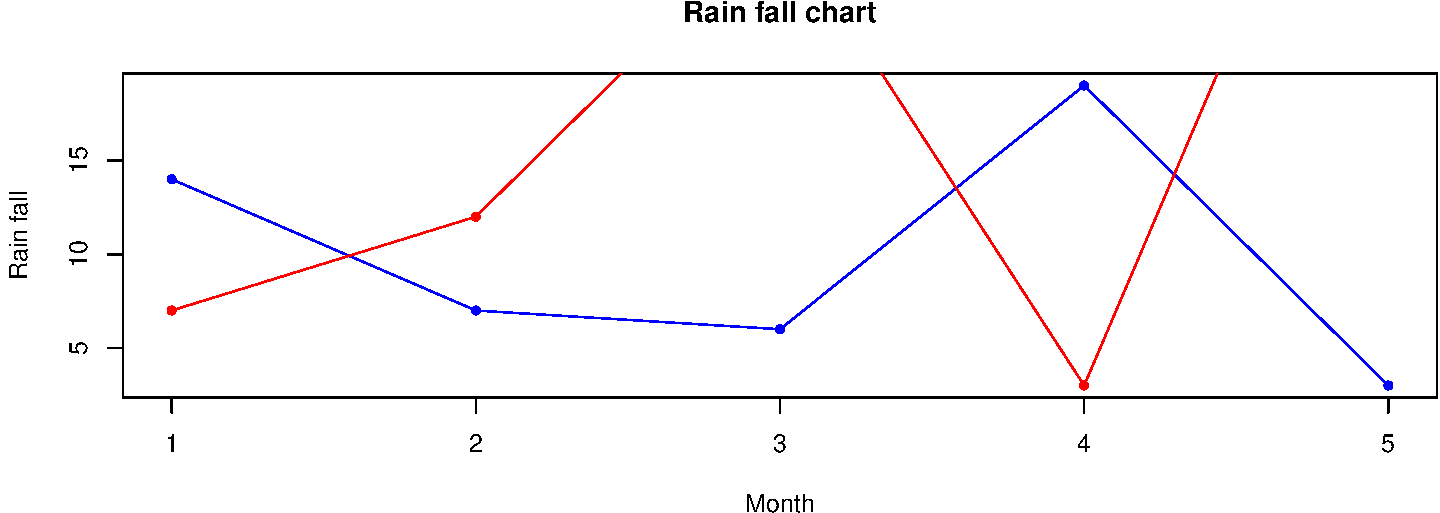
\includegraphics{/Users/lucas/Library/Mobile Documents/com~apple~CloudDocs/~~aa学习/大二上/学习/R for Data Science/R-for-Data-Science/talk06-practices_files/figure-beamer/unnamed-chunk-19-1.pdf}
\end{frame}

\begin{frame}[fragile]{把 \texttt{Others} 和 \texttt{Unknown} 放在最后}
\protect\hypertarget{ux628a-others-ux548c-unknown-ux653eux5728ux6700ux540e}{}
注意 \texttt{fct\_reorder}的用法:

\FontSmall

\begin{Shaded}
\begin{Highlighting}[]
\DocumentationTok{\#\# }
\NormalTok{abu.dat}\SpecialCharTok{$}\NormalTok{scientific\_name }\OtherTok{\textless{}{-}} 
  \FunctionTok{fct\_relevel}\NormalTok{( }\FunctionTok{fct\_reorder}\NormalTok{( abu.dat}\SpecialCharTok{$}\NormalTok{scientific\_name, abu.dat}\SpecialCharTok{$}\NormalTok{relative\_abundance, }\AttributeTok{.desc =}\NormalTok{ F),  }
               \StringTok{"Unknown"}\NormalTok{,  }\StringTok{"Others"}\NormalTok{ );}
\FunctionTok{ggplot}\NormalTok{(abu.dat, }\FunctionTok{aes}\NormalTok{(}\AttributeTok{x =}\NormalTok{ scientific\_name,}
                    \AttributeTok{y =}\NormalTok{ relative\_abundance, }\AttributeTok{fill =}\NormalTok{ scientific\_name ) ) }\SpecialCharTok{+} 
  \FunctionTok{geom\_bar}\NormalTok{( }\AttributeTok{stat =} \StringTok{"identity"}\NormalTok{ ) }\SpecialCharTok{+} 
  \FunctionTok{coord\_flip}\NormalTok{() }\SpecialCharTok{+} \FunctionTok{xlab}\NormalTok{(}\StringTok{"Species"}\NormalTok{) }\SpecialCharTok{+} \FunctionTok{ylab}\NormalTok{( }\StringTok{"Relative abundance \%"}\NormalTok{ ) }
\end{Highlighting}
\end{Shaded}

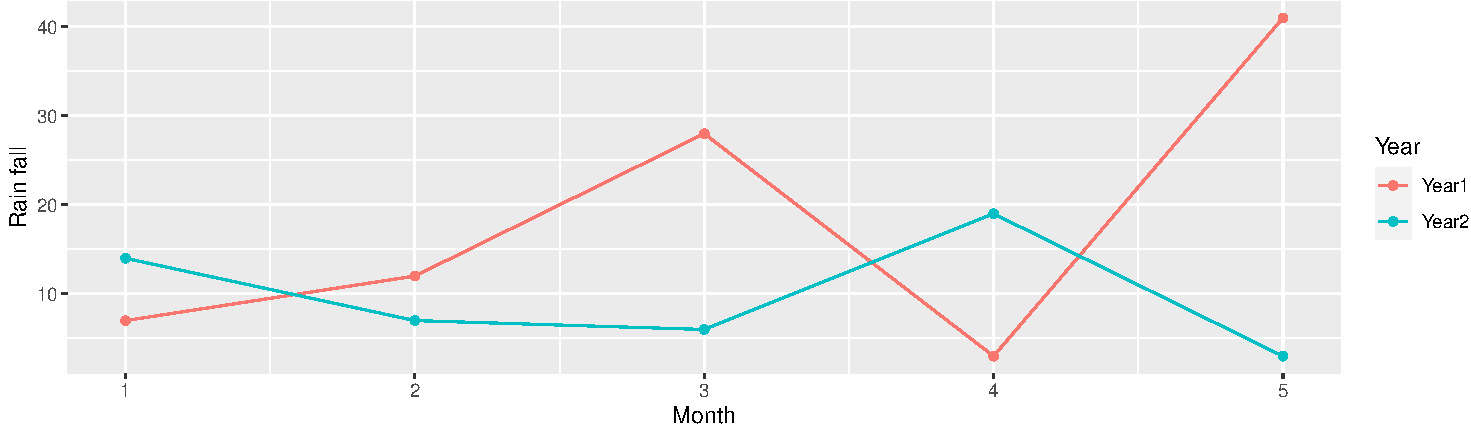
\includegraphics{/Users/lucas/Library/Mobile Documents/com~apple~CloudDocs/~~aa学习/大二上/学习/R for Data Science/R-for-Data-Science/talk06-practices_files/figure-beamer/unnamed-chunk-20-1.pdf}
\end{frame}

\begin{frame}{更多 forcats 的应用 \ldots{}}
\protect\hypertarget{ux66f4ux591a-forcats-ux7684ux5e94ux7528}{}
see here:
\url{https://cran.r-project.org/web/packages/forcats/vignettes/forcats.html}

更多应用将会在 作图 (ggplot2) 时讲到。
\end{frame}

\begin{frame}[fragile]{生信任务3 : 整合基因表达、甲基化、突变数据
(dplyr::join)}
\protect\hypertarget{ux751fux4fe1ux4efbux52a13-ux6574ux5408ux57faux56e0ux8868ux8fbeux7532ux57faux5316ux7a81ux53d8ux6570ux636e-dplyrjoin}{}
在生信分析中,常需要将多个来源的数据整合在一个表格中,以方便后续分析。

\FontSmall

\begin{Shaded}
\begin{Highlighting}[]
\NormalTok{meth }\OtherTok{\textless{}{-}} \FunctionTok{read\_delim}\NormalTok{( }\AttributeTok{file =} \StringTok{"data/talk06/methylation\_data.txt.gz"}\NormalTok{, }
                    \AttributeTok{delim =} \StringTok{"}\SpecialCharTok{\textbackslash{}t}\StringTok{"}\NormalTok{, }\AttributeTok{quote =} \StringTok{""}\NormalTok{, }\AttributeTok{col\_names =}\NormalTok{ T);}
\end{Highlighting}
\end{Shaded}

\begin{verbatim}
## Rows: 52232 Columns: 3
## -- Column specification --------------------------------------------------------
## Delimiter: "\t"
## chr (2): gene, site
## dbl (1): methylation_score
## 
## i Use `spec()` to retrieve the full column specification for this data.
## i Specify the column types or set `show_col_types = FALSE` to quiet this message.
\end{verbatim}

\begin{Shaded}
\begin{Highlighting}[]
\FunctionTok{head}\NormalTok{(meth, }\AttributeTok{n =} \DecValTok{3}\NormalTok{);}
\end{Highlighting}
\end{Shaded}

\begin{verbatim}
## # A tibble: 3 x 3
##   gene  site    methylation_score
##   <chr> <chr>               <dbl>
## 1 A1BG  1stExon             0.799
## 2 A1BG  5UTR                0.799
## 3 A1BG  Body                0.811
\end{verbatim}

\FontNormal

\textbf{问题} 什么是甲基化??
\end{frame}

\begin{frame}[fragile]{表达数据}
\protect\hypertarget{ux8868ux8fbeux6570ux636e}{}
\FontSmall

\begin{Shaded}
\begin{Highlighting}[]
\NormalTok{expr }\OtherTok{\textless{}{-}} \FunctionTok{read\_delim}\NormalTok{( }\AttributeTok{file =} \StringTok{"data/talk06/expression\_data.txt.gz"}\NormalTok{,}
                    \AttributeTok{delim =} \StringTok{"}\SpecialCharTok{\textbackslash{}t}\StringTok{"}\NormalTok{, }\AttributeTok{quote =} \StringTok{""}\NormalTok{, }\AttributeTok{col\_names =}\NormalTok{ T );}
\end{Highlighting}
\end{Shaded}

\begin{verbatim}
## Rows: 46150 Columns: 2
## -- Column specification --------------------------------------------------------
## Delimiter: "\t"
## chr (1): gene
## dbl (1): rkpm
## 
## i Use `spec()` to retrieve the full column specification for this data.
## i Specify the column types or set `show_col_types = FALSE` to quiet this message.
\end{verbatim}

\begin{Shaded}
\begin{Highlighting}[]
\FunctionTok{head}\NormalTok{( expr, }\AttributeTok{n =} \DecValTok{5}\NormalTok{);}
\end{Highlighting}
\end{Shaded}

\begin{verbatim}
## # A tibble: 5 x 2
##   gene     rkpm
##   <chr>   <dbl>
## 1 5S_RRNA     0
## 2 7SK         0
## 3 A1BG        1
## 4 A1BGAS1     4
## 5 A1CF        0
\end{verbatim}
\end{frame}

\begin{frame}{整合后的结果应该是什么??}
\protect\hypertarget{ux6574ux5408ux540eux7684ux7ed3ux679cux5e94ux8be5ux662fux4ec0ux4e48}{}
\begin{longtable}[]{@{}llllll@{}}
\toprule\noalign{}
gene & TSS200 & TSS1500 & UTR & body & expression \\
\midrule\noalign{}
\endhead
gene1 & 0.1 & 0.2 & NA & 0.8 & 100 \\
gene2 & 0.12 & 0.32 & NA & 0.9 & 18 \\
\bottomrule\noalign{}
\end{longtable}

\ldots{}
\end{frame}

\begin{frame}[fragile]{第一种方法,使用 pivot\_wider}
\protect\hypertarget{ux7b2cux4e00ux79cdux65b9ux6cd5ux4f7fux7528-pivot_wider}{}
先合并,再 pivot\_wider 用 \texttt{bind\_rows} 合并两个 tibble
时,列名需要一致

\FontSmall

\begin{Shaded}
\begin{Highlighting}[]
\NormalTok{meth2 }\OtherTok{\textless{}{-}}\NormalTok{ meth }\SpecialCharTok{\%\textgreater{}\%} \FunctionTok{select}\NormalTok{( gene, }\AttributeTok{group=}\NormalTok{site, }\AttributeTok{value=}\NormalTok{methylation\_score );}
\FunctionTok{head}\NormalTok{(meth2, }\AttributeTok{n=}\DecValTok{2}\NormalTok{);}
\end{Highlighting}
\end{Shaded}

\begin{verbatim}
## # A tibble: 2 x 3
##   gene  group   value
##   <chr> <chr>   <dbl>
## 1 A1BG  1stExon 0.799
## 2 A1BG  5UTR    0.799
\end{verbatim}

\begin{Shaded}
\begin{Highlighting}[]
\NormalTok{expr2 }\OtherTok{\textless{}{-}}\NormalTok{ expr }\SpecialCharTok{\%\textgreater{}\%} \FunctionTok{mutate}\NormalTok{( }\AttributeTok{group =} \StringTok{"rkpm"}\NormalTok{ ) }\SpecialCharTok{\%\textgreater{}\%}
  \FunctionTok{select}\NormalTok{( gene, group, }\AttributeTok{value=}\NormalTok{rkpm ) }\SpecialCharTok{\%\textgreater{}\%} 
  \FunctionTok{group\_by}\NormalTok{( gene ) }\SpecialCharTok{\%\textgreater{}\%} \FunctionTok{slice}\NormalTok{( }\DecValTok{1}\NormalTok{ );}
\FunctionTok{head}\NormalTok{(expr2, }\AttributeTok{n=}\DecValTok{2}\NormalTok{);}
\end{Highlighting}
\end{Shaded}

\begin{verbatim}
## # A tibble: 2 x 3
## # Groups:   gene [2]
##   gene    group value
##   <chr>   <chr> <dbl>
## 1 5S_RRNA rkpm      0
## 2 7SK     rkpm      0
\end{verbatim}

\FontNormal

\textbf{注:} gene name 与 group
组合必须是唯一的。即:基因A只能有一个表达量值。
\end{frame}

\begin{frame}[fragile]{合并 \& pivot\_wider}
\protect\hypertarget{ux5408ux5e76-pivot_wider}{}
\FontSmall

\begin{Shaded}
\begin{Highlighting}[]
\NormalTok{comb }\OtherTok{\textless{}{-}} \FunctionTok{bind\_rows}\NormalTok{( meth2, expr2 );}

\NormalTok{comb.wide }\OtherTok{\textless{}{-}}\NormalTok{ comb }\SpecialCharTok{\%\textgreater{}\%} \FunctionTok{pivot\_wider}\NormalTok{( }\AttributeTok{names\_from =} \StringTok{"group"}\NormalTok{, }\AttributeTok{values\_from =} \StringTok{"value"}\NormalTok{ );}

\FunctionTok{head}\NormalTok{(comb.wide);}
\end{Highlighting}
\end{Shaded}

\begin{verbatim}
## # A tibble: 6 x 8
##   gene   `1stExon` `5UTR`    Body TSS1500 TSS200 `3UTR`  rkpm
##   <chr>      <dbl>  <dbl>   <dbl>   <dbl>  <dbl>  <dbl> <dbl>
## 1 A1BG      0.799   0.799 0.811     0.852  0.850 NA         1
## 2 A1CF      0.0946  0.118 0.00798   0.110 NA     NA         0
## 3 A2M       0.899  NA     0.716     0.654 NA      0.776     1
## 4 A2ML1     0.859   0.859 0.678     0.441 NA      0.469     0
## 5 A4GALT   NA       0.844 0.821     0.890  0.513  0.814     0
## 6 A4GNT     0.680   0.680 0.538     0.402 NA     NA         0
\end{verbatim}
\end{frame}

\begin{frame}[fragile]{方法二:使用 join \ldots{}}
\protect\hypertarget{ux65b9ux6cd5ux4e8cux4f7fux7528-join}{}
首先对 methylation 数据进行处理

\FontSmall

\begin{Shaded}
\begin{Highlighting}[]
\NormalTok{meth3 }\OtherTok{\textless{}{-}} 
\NormalTok{  meth }\SpecialCharTok{\%\textgreater{}\%} \FunctionTok{pivot\_wider}\NormalTok{( }\AttributeTok{names\_from =}  \StringTok{"site"}\NormalTok{, }\AttributeTok{values\_from =} \StringTok{"methylation\_score"}\NormalTok{ );}

\FunctionTok{head}\NormalTok{(meth3);}
\end{Highlighting}
\end{Shaded}

\begin{verbatim}
## # A tibble: 6 x 7
##   gene   `1stExon` `5UTR`    Body TSS1500 TSS200 `3UTR`
##   <chr>      <dbl>  <dbl>   <dbl>   <dbl>  <dbl>  <dbl>
## 1 A1BG      0.799   0.799 0.811     0.852  0.850 NA    
## 2 A1CF      0.0946  0.118 0.00798   0.110 NA     NA    
## 3 A2M       0.899  NA     0.716     0.654 NA      0.776
## 4 A2ML1     0.859   0.859 0.678     0.441 NA      0.469
## 5 A4GALT   NA       0.844 0.821     0.890  0.513  0.814
## 6 A4GNT     0.680   0.680 0.538     0.402 NA     NA
\end{verbatim}
\end{frame}

\begin{frame}[fragile]{dplyr::join}
\protect\hypertarget{dplyrjoin}{}
\FontSmall

\begin{Shaded}
\begin{Highlighting}[]
\NormalTok{comb2 }\OtherTok{\textless{}{-}} \FunctionTok{left\_join}\NormalTok{( meth3, expr2, }\AttributeTok{by =} \StringTok{"gene"}\NormalTok{ ) }\SpecialCharTok{\%\textgreater{}\%} \FunctionTok{select}\NormalTok{( }\SpecialCharTok{{-}}\NormalTok{group );}
\FunctionTok{head}\NormalTok{(comb2)}
\end{Highlighting}
\end{Shaded}

\begin{verbatim}
## # A tibble: 6 x 8
##   gene   `1stExon` `5UTR`    Body TSS1500 TSS200 `3UTR` value
##   <chr>      <dbl>  <dbl>   <dbl>   <dbl>  <dbl>  <dbl> <dbl>
## 1 A1BG      0.799   0.799 0.811     0.852  0.850 NA         1
## 2 A1CF      0.0946  0.118 0.00798   0.110 NA     NA         0
## 3 A2M       0.899  NA     0.716     0.654 NA      0.776     1
## 4 A2ML1     0.859   0.859 0.678     0.441 NA      0.469     0
## 5 A4GALT   NA       0.844 0.821     0.890  0.513  0.814     0
## 6 A4GNT     0.680   0.680 0.538     0.402 NA     NA         0
\end{verbatim}

\FontNormal

\textbf{注意} left\_join 的语法
\end{frame}

\begin{frame}{join 详解}
\protect\hypertarget{join-ux8be6ux89e3}{}
\begin{itemize}
\item
  left\_join(): return all rows from x, and all columns from x and y.
  Rows in x with no match in y will have NA values in the new columns.
  If there are multiple matches between x and y, all combinations of the
  matches are returned.
\item
  inner\_join()
\item
  right\_join()
\item
  full\_join()
\end{itemize}

更多请见: \url{https://dplyr.tidyverse.org/reference/join.html}
\end{frame}

\hypertarget{section-3-exercise-home-work}{%
\section{section 3: Exercise \& home
work}\label{section-3-exercise-home-work}}

\begin{frame}[fragile]{练习 \& 作业}
\protect\hypertarget{ux7ec3ux4e60-ux4f5cux4e1a}{}
\begin{itemize}
\item
  \texttt{Exercises\ and\ homework} 目录下
  \texttt{talk06-practice-homework.Rmd} 文件;
\item
  完成时间:见钉群的要求
\end{itemize}
\end{frame}

\begin{frame}{小结}
\protect\hypertarget{ux5c0fux7ed3}{}
\begin{block}{今次提要}
\protect\hypertarget{ux4ecaux6b21ux63d0ux8981}{}
\begin{enumerate}
\tightlist
\item
  3个生信任务的R解决方案
\item
  factors 的更多应用 (forcats)
\end{enumerate}
\end{block}

\begin{block}{下次预告}
\protect\hypertarget{ux4e0bux6b21ux9884ux544a}{}
\begin{itemize}
\tightlist
\item
  Strings and regular expression
\end{itemize}
\end{block}

\begin{block}{important}
\protect\hypertarget{important}{}
\begin{itemize}
\tightlist
\item
  all codes are available at Github:
  \url{https://github.com/evolgeniusteam/R-for-bioinformatics}
\end{itemize}
\end{block}
\end{frame}

\end{document}